
\chapter{Алгоритмы оценки состояния}
\label{chapter_estimation}

Для реализации обратных связей в контуре управления необходимо обеспечить оценку текущего положения, скорости, кватерниона ориентации и угловой скорости БЛА. Получить эти данные можно с помощью стандартного набора бортовых датчиков, обычно включающий себя спутниковую систему глобального позиционирования, цифровой барометрический датчик давления, трехосевые электромеханические акселерометр и гироскоп, а также магнитный компас. Однако, в связи с высокими требованиями к массово-габаритным параметрам бортовой системы навигации для небольших летательных аппаратов, бортовые измерения имеют ограничения по качеству. Высокий уровень шума побуждает использовать численные методы нелинейной фильтрации, с помощью которых можно значительно повысить качество оценки состояния БЛА.

На первом этапе разработки системы управления квадрокоптером с поворотными роторами для оценки состояния использовался расширенный фильтр Калмана. Однако, как известно, реализация этого фильтра существенно полагается на предположение о том, что линеаризованное преобразование математического ожидания вектора состояния системы и соответствующей матрицы ковариации достаточно близко к истинному нелинейному преобразованию, определяемому динамикой системы. В связи с этим для нелинейных систем, какой является динамика квадрокоптера с поворотными роторами, производительность алгоритма расширенного фильтра Калмана (extended Kalman filter, EKF) может снижаться.
Для выбора подходящего алгоритма фильтрации проведено исследование \cite{Shavin02}, где помимо EKF рассмотрены несколько вариантов реализации сигма-точечного фильтра Калмана (unscented Kalman filter, UKF) \cite{Julier01, Julier02}. Преимуществом этого метода является более высокая точность аппроксимации при тех же вычислительных затратах, что и в EKF-методе \cite{Kulikova01}. Кроме того, как показывают численные эксперименты \cite{Shavin01}, стандартный алгоритм расширенного фильтра Калмана более чувствителен к ошибкам дискретизации и округления, чем некоторые частные реализации сигма-точечного фильтра Калмана. Ниже будет приведено описание принципов работы EKF, UKF, а также одной из частных реализаций сигма-точечного фильтра -- кубатурного фильтра Калмана (cubature Kalman filter, CKF) и описаны особенности применения этих алгоритмов для оценки состояния квадрокоптера с поворотными роторам.


%% EKF
\section{Расширенный фильтр Калмана}

Расширенный фильтр Калмана использует модель непрерывной динамической системы
\begin{equation} \label{eq:ekf_system}
\dot{\bm{x}} = f(\bm x, t) + \bm w,
\end{equation}
и дискретные измерения
\begin{equation} \label{eq:ekf_mes}
\bm z_k = h_k(\bm x(t_k)) + \bm y_k.
\end{equation}
Здесь, $\bm x$ -- вектор состояния системы, в данном случае
\begin{equation} \label{eq:ekf_state}
\bm x = (\bm r^I, \bm v^I, q_{IB},\bm \Omega^B);
\end{equation}
$\bm w$ -- шум системы, $\bm y_k$ -- шум измерений.
Задача фильтрации — найти являющуюся функцией измерений
$\bm z_k$
оценку вектора состояния системы
$\bm x(t_k)$,
минимизирующую среднеквадратичную ошибку
\begin{equation}
E\left\langle {{{\left[ {{{{\bm{\hat x}}}_k} - {{\bm{x}}_k}} \right]}^T}{\bm{M}}\left[ {{{{\bm{\hat x}}}_k} - {{\bm{x}}_k}} \right]} \right\rangle
\end{equation}
Эту оценку обозначим $\hat{\bm{x}}_k$.
Пусть в момент времени $t_{k-1}$ получена оценка вектора состояния
$\hat{\bm{x}}_{k-1}$.
На основании этой оценки строится прогноз оценки вектора состояний
$\hat{\bm{x}}_k^-$
(оценка априори), затем проводятся измерения
$\bm z_k$
и коррекция оценки априори на основании результатов измерений
$\hat{\bm{x}}_k^+$
(оценка апостериори). Оценку априори вектора состояния
$\hat{\bm{x}}_k^-$ вычисляют интегрированием модельного уравнения
\begin{equation}
\frac{d\hat{\bm{x}}}{dt} = f(\hat{\bm{x}}, t)
\end{equation}
с начальными условиями
$\hat{\bm{x}}(t) = \hat{\bm{x}}_{k-1}, \quad \hat{\bm{x}}(0) = \bm x_0$.
Оценку априори ковариационной матрицы ошибки для линеаризованных уравнений в приращениях
$\bm P_k^-$
вычисляют как
\begin{equation}
\bm P_k^- = \bm \Phi \bm P_{k-1}^+ \bm \Phi^{T} + \bm Q
\end{equation}
\begin{equation}
\bm F = \frac{\partial f(\bm x, t)}{\partial \bm x} \Bigg|_{\bm{x} = \hat{\bm{x}}_{k-1}}
, \quad
\bm \Phi = \bm E + \bm F \Delta t
\end{equation}
с начальными условиями
$\hat{\bm{P}}(t) = \bm{P}_{k-1}^+, \quad \bm{P}(0) = \bm P_0$.
Здесь, $\bm Q$ -- ковариационная матрица шума системы. Оценку апостериори для вектора состояния и ковариационной матрицы ошибки строят следующим образом:
\begin{equation}
\begin{array}{l}
{\bm{\hat x}}_k^ +  = {\bm{\hat x}}_k^ -  + {{\bm{K}}_k}({{\bm{z}}_k} - {{\bm{H}}_k}{\bm{\hat x}}_k^ - ),\\
{\bm{P}}_k^ +  = \left( {{\bm{I}} - {{\bm{K}}_k}{{\bm{H}}_k}} \right){\bm{P}}_k^ - .
\end{array}
\end{equation}
${{\bm{H}}_k}$ -- линеаризованная матрица чувствительности:
\begin{equation}
{\bm{H}}_k = \frac{\partial {h}({\bm{x}},t)}{\partial {\bm{x}}} \Bigg|_{\bm x = {{\bm{\hat x}}_{k - 1}}},
\end{equation}
а ${{\bm{K}}_k}$ -- корректирующая матрица обратной связи --
$${{\bm{K}}_k} = {\bm{P}}_k^ - \,{\bm{H}}_k^T{\left[ {{{\bm{H}}_k}\,{\bm{P}}_k^ - \,{\bm{H}}_k^T + {{\bm{R}}_k}} \right]^{ - 1}},$$
где $\bm R$ -- ковариационная матрица шума измерений. Описанный в начале этого параграфа набор бортовых датчиков может обеспечить измерения входящих в вектор состояния величин, тогда вектор измерений
\begin{equation} \label{eq:ukf_mes}
\bm z = (\bm r^I, \bm v^I, q_{IB},\bm \Omega^B).
\end{equation}

Линеаризация упрощенной модели \eqref{eq:m_dyn} приводит к следующему выражению для матрицы $\bm F$:
\begin{equation}
{\bm{F}} =
\left( {\begin{array}{*{20}{c}}
	{{{\bm{O}}_{3\times3}}}&{{{\bm{E}}_{3\times3}}}&{{{\bm{O}}_{3\times4}}}&{{{\bm{O}}_{3\times3}}}\\
	{{{\bm{O}}_{3\times3}}}&{{\bm{M}}_{3\times3}^1}&{{\bm{M}}_{3\times4}^2}&{{{\bm{O}}_{3\times3}}}\\
	{{{\bm{O}}_{4\times3}}}&{{{\bm{O}}_{4\times3}}}&{{\bm{M}}_{4\times4}^3}&{\frac{1}{2}\left[ {\begin{array}{*{20}{c}}
			{{{\bm{O}}_{3\times1}}}&{{{\bm{E}}_{3\times3}}}
			\end{array}} \right]}\\
	{{{\bm{O}}_{3\times3}}}&{{{\bm{O}}_{3\times3}}}&{{{\bm{O}}_{3\times4}}}&{{\bm{M}}_{3\times3}^4}
	\end{array}} \right),
\end{equation}
где
\begin{equation}
{{\bm{M}}_{3x3}^1 =  - \frac{{\rho C{S_ \bot }}}{{2M}}\left| {\bm{v}} \right|\left( {{{\bm{E}}_{3x3}} + \frac{{{\bm{v}} \cdot {{\bm{v}}^T}}}{{{{\left| {\bm{v}} \right|}^2}}}} \right)}
\end{equation}
\vspace{3mm}
\begin{equation}
{{\bm{M}}_{3x4}^2 =  - \frac{2}{M}\left( {\begin{array}{*{20}{c}}
		{{{\bm{O}}_{3x1}}}&{{{\left[ {{{\bm{Q}}_{IB}}{\bm{f}}_{\ddot r}^B({\bm{\theta }},{\bm{\tilde \omega }})} \right]}_ \times }}
		\end{array}} \right)},
\end{equation}
\vspace{3mm}
\begin{equation}
{\bm{M}}_{4x4}^3 =  - \left( {\begin{array}{*{20}{c}}
	0&{{{\bm{O}}_{1x3}}}\\
	{{{\bm{O}}_{3x1}}}&{{{[{{\bm{\Omega }}^B}]}_ \times }}
	\end{array}} \right),
\end{equation}
\vspace{3mm}
\begin{equation}
{{\bm{M}}_{3x3}^4 = {\bm{J}}_B^{ - 1}\left( {{{\left[ {{{\bm{J}}_B}{{\bm{\Omega }}^B}} \right]}_ \times } - {{\left[ {{{\bm{\Omega }}^B}} \right]}_ \times }{{\bm{J}}_B}} \right)},
\end{equation}
где символом ${\left[ {...} \right]_ \times }$  обозначен кососимметрический оператор векторного произведения,
${{{\bm{O}}_{n\times m}}}$ и ${{{\bm{E}}_{n\times m}}}$ -- нулевая и единичная матрицы размерности $n \times m$.

Матрица чувствительности имеет тривиальный вид
\begin{equation}
{\bm{H}} =
\left( {\begin{array}{*{20}{c}}
	{{{\bm{E}}_{3x3}}}&{{{\bm{O}}_{3x3}}}&{{{\bm{O}}_{3x4}}}&{{{\bm{O}}_{3x3}}}\\
	{{{\bm{O}}_{3x3}}}&{{{\bm{E}}_{3x3}}}&{{\bm{O}}_{3x4}}&{{{\bm{O}}_{3x3}}}\\
	{{{\bm{O}}_{4x3}}}&{{{\bm{O}}_{4x3}}}&{{{\bm{E}}_{4x4}}}&{{{\bm{O}}_{4x3}}}\\
	{{{\bm{O}}_{3x3}}}&{{{\bm{O}}_{3x3}}}&{{{\bm{O}}_{3x4}}}&{{{\bm{E}}_{3x3}}}
	\end{array}} \right).
\end{equation}

\section{Сигма-точечный фильтр Калмана}

Сигма-точечный фильтр Калмана является модификацией стандартного алгоритма, ключевой особенностью которого является отсутствие необходимости линеаризовывать модель \eqref{eq:ekf_system} непрерывной динамической системы. Алгоритм использует модель дискретных измерений \eqref{eq:ekf_mes}.
Задача фильтрации -- найти являющуюся функцией измерений $\bm z_k$ несмещенную оценку вектора состояния системы  $\bm x(t_k)$, минимизирующую дисперсию ошибки  ${\hat{\bm{x}}_k} - \bm x({t_k})$.
Априори оценка вектора состояния $\bm{\hat x}_k^-$ вычисляется как
\begin{equation} \label{eq:ukf_apr}
{\bm{\hat x}}_k^-  = \sum\limits_{i = 0}^{2N} {{w^i} \cdot } \,f\left( {{\bm{X}}_k^i} \right),
\end{equation}
Аргументами функции $f$ в выражении \eqref{eq:ukf_apr} являются так называемые сигма-точки, выбор которых определяется соотношениями
\begin{equation} \label{eq:ukf_points}
\begin{aligned}
&{{\bm{X}}_k^0 = {{\bm{x}}_{k - 1}}},
\\
&{{\bm{X}}_k^i = {{\bm{x}}_{k - 1}} + \sqrt {N + {{\lambda }}}  \cdot {{\left( {\sqrt {{{\bm{P}}_{k - 1}}} } \right)}^i}}, \quad {i = 1,...,N}
\\
&{{\bm{X}}_k^i = {{\bm{x}}_{k - 1}} + \sqrt {N + {{\lambda }}}  \cdot {{\left( {\sqrt {{{\bm{P}}_{k - 1}}} } \right)}^{i - N}}}, \quad {i = N + 1,...,2N}
\end{aligned}
\end{equation}
где
${{{\left( {\sqrt {{{\bm{P}}_{k - 1}}} } \right)}^i}}$
обозначает  $i$-й столбец матрицы ${\sqrt {{{\bm{P}}_{k - 1}}} }$.  Здесь используется разложение Холецкого \cite{Verbjitsky01} вида
${\bm{P}} = \sqrt {\bm{P}} {\sqrt {\bm{P}} ^T},$
где $\sqrt {\bm{P}}$ -- нижняя треугольная матрица. $N$ -- размерность оцениваемого вектора состояния. Весовые коэффициенты в формуле \eqref{eq:ukf_apr} вычисляются как
\begin{equation} \label{eq:ukf_weights}
{w^0} = \frac{{{\lambda }}}{{{{\lambda }} + N}},
\quad
{w^i} = \frac{1}{{2\left( {{{\lambda }} + N} \right)}},
\quad
i = 1,...,2N.
\end{equation}
Оценка матрицы ковариации может быть получена по формуле
\begin{equation} \label{eq:ukf_p_apr}
{\bm{P}}_k^ -  = \sum\limits_{i = 0}^{2N} {{w^i}\left( {f\left( {{\bm{X}}_k^i} \right) - {\bm{\hat x}}_k^ - } \right)} {\left( {f\left( {{\bm{X}}_k^i} \right) - {\bm{\hat x}}_k^ - } \right)^{{T}}} + {\bm{Q}},
\end{equation}
где $\bm{Q}$ -- ковариационная матрица шума системы.
При этом весовые коэффициенты в формулах \eqref{eq:ukf_apr} и \eqref{eq:ukf_p_apr} совпадают за исключением коэффициента  ${w^0}$, который в формуле \eqref{eq:ukf_p_apr} принимает значение \cite{Kulikova01}
\begin{equation}
w^0 = \frac{{{\lambda }}}{{{{\lambda }} + N}} + 1 - {{{\alpha }}^2} + {{\beta }},
\end{equation}
где
${{\alpha }} \in \left[ {{{10}^{ - 4}},1} \right]$
-- параметр, определяющий разброс сигма-точек вокруг среднего.
Параметр ${{\beta }}$  позволяет учесть априорные данные о функции плотности вероятности неизвестного вектора состояния системы (для нормального распределения  ${{\beta }} = 2$). Наконец, ${{\lambda }} = {\alpha }^2 (N + \kappa) - N$ -- параметр масштабирования.
Далее происходит коррекция сделанных на предыдущем этапе оценок вектора состояния и матрицы ковариации с помощью вектора и модели измерений.
С помощью функции $h$ из уравнений \eqref{eq:ekf_mes} сигма-точки \eqref{eq:ukf_points} отображаются в пространство измерений, где также делается оценка среднего и матрицы ковариации
\begin{equation}
{\bm{\zeta }}_k^i = h\left( {{\bm{X}}_k^i} \right),
\end{equation}
\begin{equation}
{{{\bm{\hat z}}}_k} = \sum\limits_{i = 0}^{2N} {{w^i} \cdot } \,{\bm{\zeta }}_k^i,
\end{equation}
\begin{equation} \label{eq:ukf_s_k}
{{\bm{S}}_k} = \sum\limits_{i = 0}^{2N} {{w^i}\left( {{\bm{\zeta }}_k^i - {{{\bm{\hat z}}}_k}} \right)} {\left( {{\bm{\zeta }}_k^i - {{{\bm{\hat z}}}_k}} \right)^{{T}}} + {\bm{R}},
\end{equation}
где $\bm R$ -- ковариационная матрица шума измерений. Окончательные оценки для вектора состояния и матрицы ковариации получаются по формулам
\begin{equation}
{\bm{\hat x}}_k^ +  = {\bm{\hat x}}_k^ -  + {{\bm{K}}_k}({{\bm{z}}_k} - {{{\bm{\hat z}}}_k}),
\end{equation}
\begin{equation}
{\bm{P}}_k^ +  = \left( {{\bm{E}} - {{\bm{K}}_k}{{\bm{T}}_k}} \right){\bm{P}}_k^ - ,
\end{equation}
где
\begin{equation}
{{\bm{T}}_k} = \sum\limits_{i = 0}^{2N} {{w^i}\left( {{\bm{X}}_k^i - {\bm{\hat x}}_k^ - } \right)} {\left( {{\bm{\zeta }}_k^i - {{{\bm{\hat z}}}_k}} \right)^{{T}}},
\end{equation}
\begin{equation}
{{\bm{K}}_k} = {{\bm{T}}_k}{\bm{S}}_k^{ - 1}.
\end{equation}
Таким образом, алгоритм сигма-точечного фильтра Калмана имеет три параметра $\alpha$, $\beta$ и $\kappa$, выбор которых определяет конкретную UKF-реализацию.

\section{Кубатурный фильтр Калмана}
Кубатурный фильтр Калмана разработан в 2000 году и избавлен от
проблемы быстро растущей вычислительной сложности квадратурных фильтров \cite{Arasaratnam}.
В кубатурном фильтре используется кубатурное правило Гаусса третьего порядка для
оценки математического ожидания производной вектора состояния
\begin{equation*}
\mathbb{E}[f(x)] = \int_{\mathbb{R}^N}^{} f(x) \Upsilon(x, \mu, \Sigma) dx \approx \frac{1}{2N} \sum_{i=1}^{2N}f(\mu + \sqrt \Sigma \zeta_i),
\end{equation*}
где $\Upsilon(x, \mu, \Sigma)$ -- функция плотности вероятностинормального распределения случайного вектора $x$
со средним $\mu$ и ковариацией $\Sigma = \sqrt \Sigma \sqrt{\Sigma}^T$, $\zeta$ - узлы кубатурной функции
\begin{equation*}
\zeta =
\begin{cases}
\sqrt N e_i, & \quad i = 1,...,N,\\
-\sqrt N e_{i-N}, &\quad i = N+1,...,2N,
\end{cases}
\end{equation*}
где $e_i$ -- $i$-ый координатный вектор пространства $\mathbb R^N$.
Нетрудно обнаружить, что  выбор параметров сигма-точечного фильтра Калмана
$\alpha=1$, $\beta=0$, $\kappa=0$
соответствует реализации кубатурного фильтра Калмана,
так как весовые коэффициенты (\ref{eq:ukf_weights})
и выражения для математического ожидания и ковариации с учетом предположения
о нормальности распределения вектора состояния в этом случае совпадают.
Таким образом, CKF в каком-то смысле является частной реализацией UKF.

\section{Сравнение производительности алгоритмов}

Для сравнения производительности описанных выше методов проведены вычислительные эксперименты.
Предложенные в главе \ref{chapter_dyn} алгоритмы использовались для управления БЛА, в качестве целевых траекторий выбраны трехмерные кривые в пространстве, параметры которых генерировались случайным образом в известных пределах.

В качестве параметра, определяющего производительность фильтров,
выбрано среднеквадратичное отклонение компонент вектора оценки состояния от результатов интегрирования уравнений движения.
Для исключения влияния параметров конкретной целевой траектории на результаты эксперимента
среднеквадратичное отклонение усредняется по 100 однотипным траекториям.
Длительность каждого полетного задания составляет 90 секунд, в течение этого времени квадрокоптер
двигается по криволинейной траектории в пространстве,
а его корпус разворачивается согласно целевым параметрам ориентации в текущий момент.
Максимальная допустимая скорость аппарата ограничена значением 5 м/с,
а угловая скорость -- $3^\circ$/c. Все три фильтра используют одинаковые измерения
и работают на одном и том же наборе траекторий.

Измерения моделируются добавлением к результатам интегрирования уравнений движения (\ref{eq:m_dyn}) белого гауссовского шума, параметры которого выбраны таким образом, чтобы соответствовать параметрам существующих устройств \cite{xsens01}.


\begin{table}[h!]
	\caption{ -- Параметры шума измерений}\label{tb:est_noise_params} 
	\centering
	\begin{tabular}{|>
			{\centering\arraybackslash}m{1.5in}|>
			{\centering\arraybackslash}m{1.5in}|}
		\hline
		${{{\sigma }}_{rx}}$& 1м \\ \hline
		${{{\sigma }}_{rz}}$& 2м \\ \hline
		${{{\sigma }}_{v}}$& 0.5м/с \\ \hline
		${{{\sigma }}_{\alpha}}$& 0.5$^\circ$ \\ \hline
		${{{\sigma }}_{\beta}}$& 0.5$^\circ$ \\ \hline
		${{{\sigma }}_{\gamma}}$& 1.5$^\circ$ \\ \hline
		${{{\sigma }}_{\Omega}}$& 0.6$^\circ$/c \\ \hline
	\end{tabular}
\end{table}

Стандартные отклонения шума измерений горизонтальных компонент положения, вертикальной компоненты позиции, компонент скорости, углов тангажа, крена, рысканья и компонент угловой скорости приведены в табл. 1.

В качестве модели динамики летательного аппарата в алгоритмах нелинейной фильтрации используется упрощенная модель движения квадрокоптера, в которой не учтена инерция поворотных роторов с пропеллерами. Тогда, выражение для углового ускорения (\ref{eq:m_dyn}) запишется, как
\begin{equation*} \label{eq:model}
\begin{aligned}
&\dot{\bm \Omega} =
{\bm J}_B^{-1}\Big[
- {\bm \Omega} \times {\bm J}_B{{\bm \Omega}}
+
\sum_{i=1}^{4} {{\bm r}^B_i \times(-1)^{i+1} k \tilde \omega_i |\tilde \omega_i| {\bm e}^I_{z_i}}
- 
\sum_{i=1}^{4}{q_{B {R_i}} \circ{b \tilde \omega_i |\tilde \omega_i| \bm e^{R_i}_{r_i}}\circ \tilde q_{ B {R_i}}}
\Big].
\end{aligned}
\end{equation*}
К данному упрощению часто прибегают на практике,
так как при проектировании квадрокоптера с поворотными роторами даже приблизительная идентификация основных
параметров динамики исполнительных органов системы управления является трудоемким процессом и требует проведения специальных измерений \cite{Ryll01}.
Таким образом, выражения, связанные с динамикой исполнительных органов системы управления формирует вектор $w$ шума системы из уравнения стохастической непрерывной системы \eqref{eq:m_dyn}.

Производительность каждого из алгоритмов фильтрации исследуется для различных интервалов наблюдения,
кратных шагу интегрирования системы,
то есть измерения и оценка состояния производятся с интервалами $T_N = N\delta$.

Матрицы $Q$ ковариации шума системы и $R$ ковариации шума измерений,
используемые во всех трех алгоритмах,
выбраны с учетом знаний о параметрах шума измерений
и скорректированы таким образом, чтобы алгоритмы показывали
высокую производительность для интервала измерений $T_1 = \delta$:
\begin{equation*} \label{eq:QR}
\begin{aligned}
&Q = 10^{-6} diag(1,\ 1,\ 1,\ 1,\ 1,\ 1,\ 1,\ 1,\ 1,\ 1,\ 50,\ 50,\ 50),\\
&R = diag(1,\ 1,\ 1,\ 0.5,\ 0.5,\ 0.5,\ 0.003,\
0.003,\ 0.003,\ 0.006,\ 0.003,\ 0.003,\ 0.003).
\end{aligned}
\end{equation*}

Результаты численных экспериментов представлены в табл. \ref{tb:est_cmpr},
где приведены значения усредненных по 100 пролетам среднеквадратичных
отклонений оценки состояния
и количество случаев некорректной оценки.
Некорректной оценкой считается случай, когда ее качество становится хуже, чем качество измерений (табл.1),
такие результаты не учитывались при усреднении.
Таблица не содержит $y$-компонент элементов вектора состояния,
так как эти результаты качественно не отличаются от параметров для $x$-компоненты.


\begin{table}[h!]
\small
	\caption{ -- Сравнение производительности алгоритмов фильтрации}\label{tb:est_cmpr} 
	\centering
	\begin{tabular}{>
			{\centering\arraybackslash}m{0.3in}|>
			{\centering\arraybackslash}m{0.5in}|>
			{\centering\arraybackslash}m{0.5in}|>
			{\centering\arraybackslash}m{0.5in}|>
			{\centering\arraybackslash}m{0.5in}|>
			{\centering\arraybackslash}m{0.5in}|>
			{\centering\arraybackslash}m{0.5in}|>
			{\centering\arraybackslash}m{0.5in}|>
			{\centering\arraybackslash}m{0.5in}|>
			{\centering\arraybackslash}m{0.5in}}
		\hline
		
		$N$       &Метод    &$r_x$,м     &$r_z$,м       &$v_x$,м/с      &$v_z$,м/с       &$e_x$,$^\circ$      &$e_z$,$^\circ$     &$o_x$,$^\circ$/c     &$o_z$,$^\circ$/c \\ \hline
		&EKF    &0.14/0       &0.13/0     &0.07/0     &0.02/0     &0.14/0     &0.11/0     &0.27/0    &0.23/0    \\              
		1 &UKF    &0.10/0       &0.19/0     &0.06/0     &0.06/0     &0.18/0     &0.21/0     &0.30/0    &0.23/0    \\              
		&CKF    &0.09/0       &0.14/0     &0.06/0     &0.03/0     &0.15/0     &0.21/0     &0.28/0    &0.23/0    \\ \hline       
		&EKF    &0.48/0       &0.23/0     &0.17/0     &0.04/0     &0.22/0     &0.17/0     &0.30/0    &0.23/0    \\              
		2 &UKF    &0.16/0       &0.26/0     &0.09/0     &0.09/0     &0.27/0     &0.27/0     &0.36/0    &0.22/0    \\              
		&CKF    &0.14/0       &0.17/0     &0.09/0     &0.03/0     &0.24/0     &0.27/0     &0.33/0    &0.22/0    \\ \hline       
		&EKF    &0.80/53      &0.63/22    &0.29/0     &0.16/0     &0.25/0     &0.22/0     &0.33/0    &0.22/0    \\              
		3 &UKF    &0.19/0       &0.33/0     &0.10/0     &0.11/0     &0.33/0     &0.31/0     &0.40/0    &0.22/0    \\              
		&CKF    &0.18/0       &0.22/0     &0.10/0     &0.03/0     &0.30/0     &0.31/0     &0.35/0    &0.22/0    \\ \hline       
		&EKF    &0.96/99      &0.82/89    &0.40/27    &0.31/9     &0.31/7     &0.29/0     &0.33/0    &0.25/0    \\              
		4 &UKF    &0.23/0       &0.39/0     &0.13/0     &0.13/0     &0.43/6     &0.35/0     &0.40/0    &0.24/0    \\              
		&CKF    &0.21/0       &0.24/0     &0.13/0     &0.04/0     &0.40/0     &0.36/0     &0.36/0    &0.24/0    \\ \hline       
		&EKF    &$\infty$/100      &$\infty$/100    &0.37/67    &0.37/68    &0.33/21    &0.29/0     &0.34/0    &0.25/0    \\              
		5 &UKF    &0.23/0       &0.40/0     &0.12/0     &0.14/0     &0.44/25    &0.37/0     &0.40/0    &0.24/0    \\              
		&CKF    &0.19/0       &0.25/0     &0.12/0     &0.06/0     &0.43/6     &0.37/0     &0.37/0    &0.24/0    \\ \hline       
		&EKF    &$\infty$/100      &$\infty$/100    &0.37/73    &0.40/88    &0.37/19    &0.32/0     &0.37/0    &0.23/0    \\              
		6 &UKF    &0.29/0       &0.48/0     &0.15/0     &0.16/0     &0.44/25    &0.40/0     &0.42/0    &0.23/0    \\              
		&CKF    &0.26/0       &0.31/0     &0.15/0     &0.05/0     &0.40/1     &0.41/0     &0.40/0    &0.22/0    \\ \hline       
		&EKF    &$\infty$/100      &$\infty$/100    &0.40/76    &0.42/98    &0.49/99    &0.58/1     &0.40/0    &0.28/0    \\              
		7 &UKF    &0.27/0       &0.50/0     &0.15/0     &0.17/0     &0.47/81    &0.40/0     &0.40/0    &0.26/0    \\              
		&CKF    &0.23/0       &0.31/0     &0.15/0     &0.06/0     &0.45/52    &0.40/0     &0.41/0    &0.25/0    \\ \hline       
		&EKF    &0.85/99      &$\infty$/100    &0.38/86    &0.38/85    &0.46/79    &0.37/0     &0.38/0    &0.27/0    \\              
		8 &UKF    &0.30/0       &0.53/0     &0.17/0     &0.16/0     &0.46/71    &0.44/0     &0.41/0    &0.28/0    \\              
		&CKF    &0.27/0       &0.37/0     &0.16/0     &0.07/0     &0.45/41    &0.45/0     &0.45/0    &0.27/0    \\ \hline       
		&EKF    &$\infty$/100      &$\infty$/100    &0.44/96    &0.38/88    &$\infty$/100    &0.69/16    &0.44/4    &0.31/3    \\              
		9 &UKF    &0.30/0       &0.52/0     &0.15/0     &0.19/0     &$\infty$/100    &0.45/0     &0.44/0    &0.28/0    \\              
		&CKF    &0.26/0       &0.27/0     &0.15/0     &0.08/0     &0.49/94    &0.48/0     &0.49/2    &0.27/0    \\ \hline 
	\end{tabular}
\normalsize
\end{table}


Как и ожидалось, качество оценки вектора состояния зависит от величины интервала работы фильтра --
снижение частоты измерений ведет к ухудшению параметров оценки.
Наиболее низкую производительность на больших интервалах измерений показывает расширенный фильтр Калмана:
уже для $N>2$ ошибки оценки состояния в нескольких случаях выходят за рамки допустимых,
а при $N \geq 5$ оценка положения становится некорректной.
Производительность сигма-точечного и кубатурного фильтров Калмана с ростом $N$ также падает,
но не настолько заметно, при этом отказов в работе этих алгоритмов значительно меньше.
Сравнительный анализ результатов UKF и CKF показал, что CKF-алгоритм производит более точную оценку состояния
в большинстве рассматриваемых случаев и является более устойчивым к повышению интервала измерений.
На рис. \ref{fig:est_cmpr} изображены графики зависимости среднеквадратичных отклонений
$z$-компонент вектора оценки состояния от временных интервалов измерений.
\begin{figure}[h]
	\begin{minipage}[h]{0.49\linewidth}
		\center{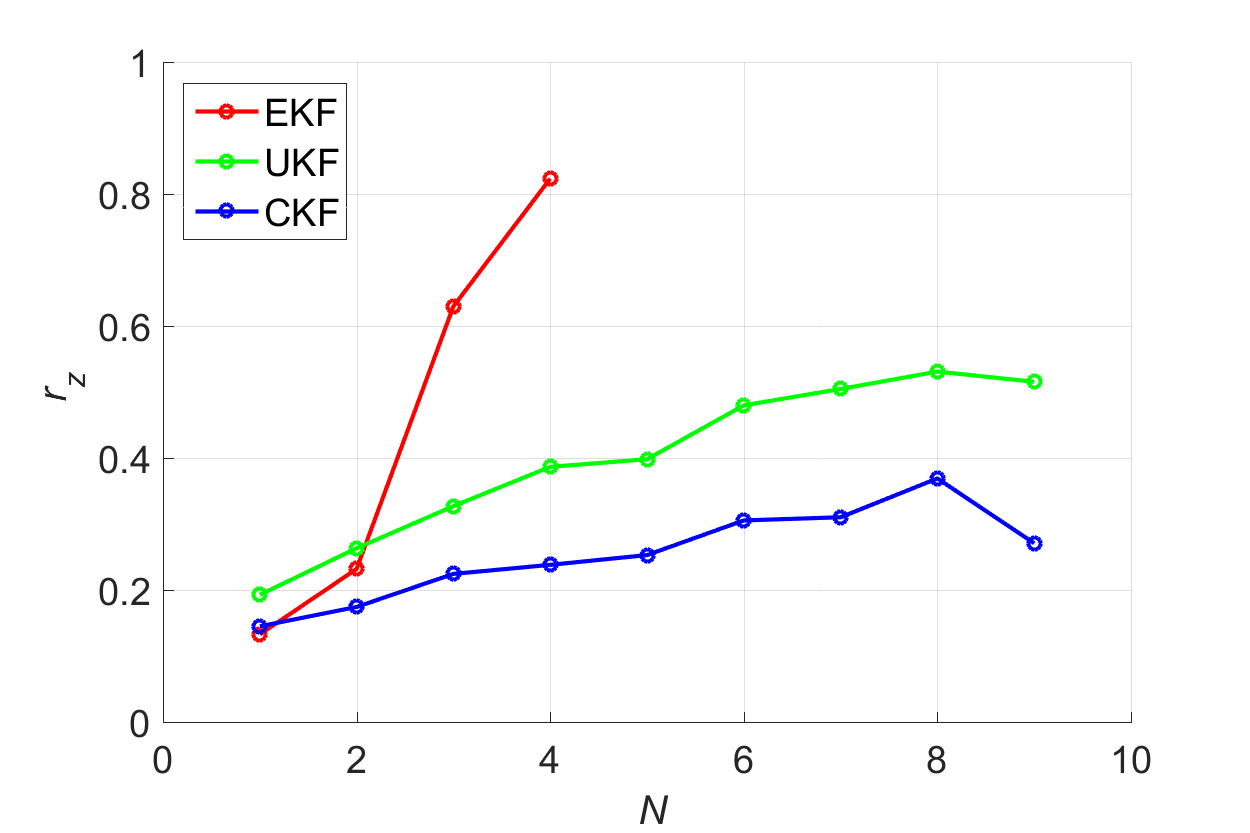
\includegraphics[height=0.2\textheight]{estcmpr_1} \\ а)}
	\end{minipage}
	\hfill
	\begin{minipage}[h]{0.49\linewidth}
		\center{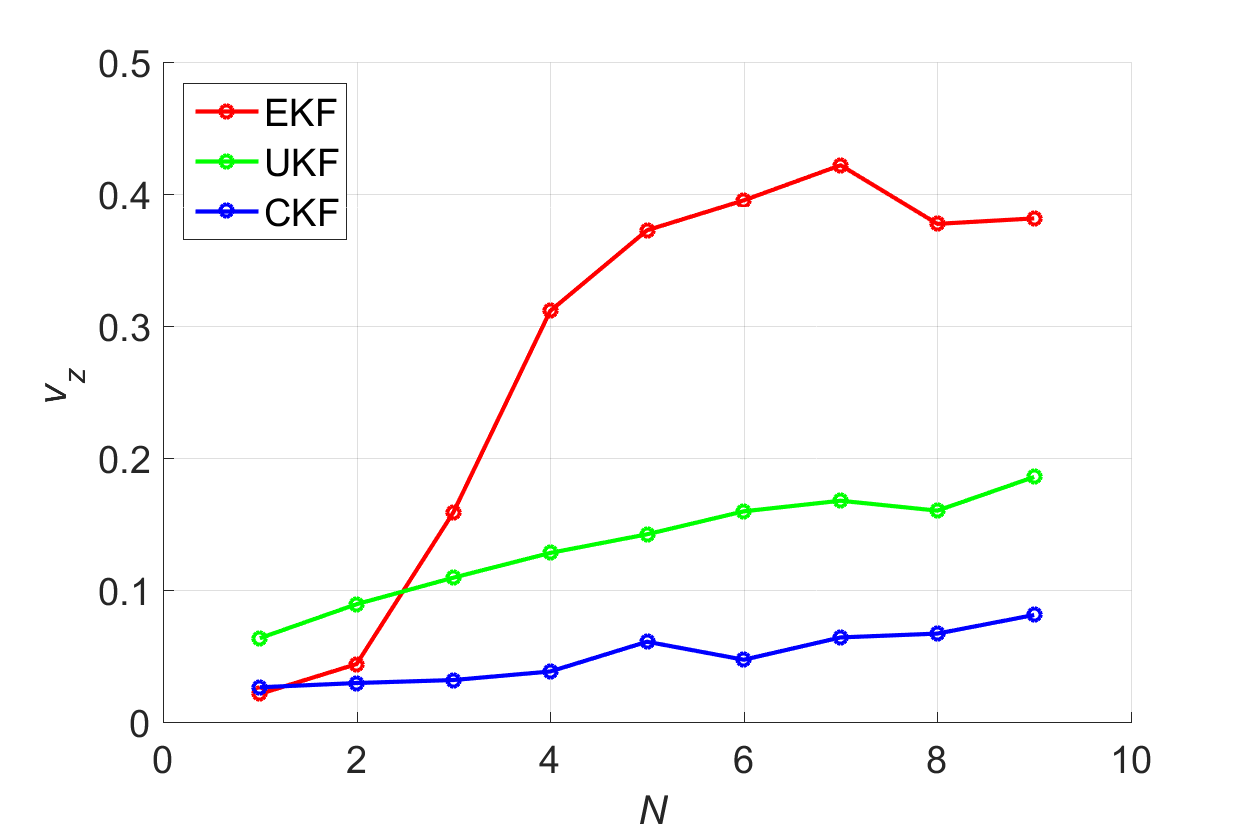
\includegraphics[height=0.2\textheight]{estcmpr_2} \\ б)}
	\end{minipage}
	\\
	\begin{minipage}[h]{0.49\linewidth}
		\center{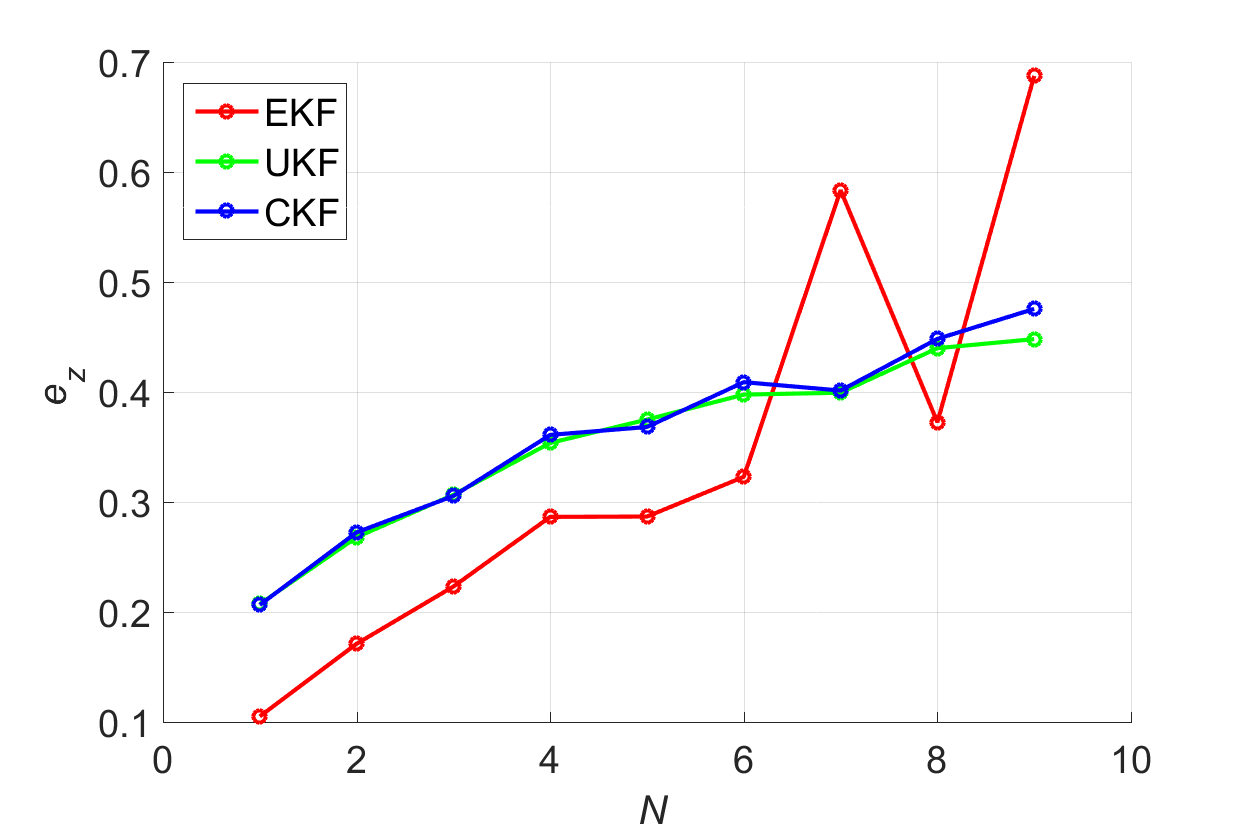
\includegraphics[height=0.2\textheight]{estcmpr_3} \\ а)}
	\end{minipage}
	\hfill
	\begin{minipage}[h]{0.49\linewidth}
		\center{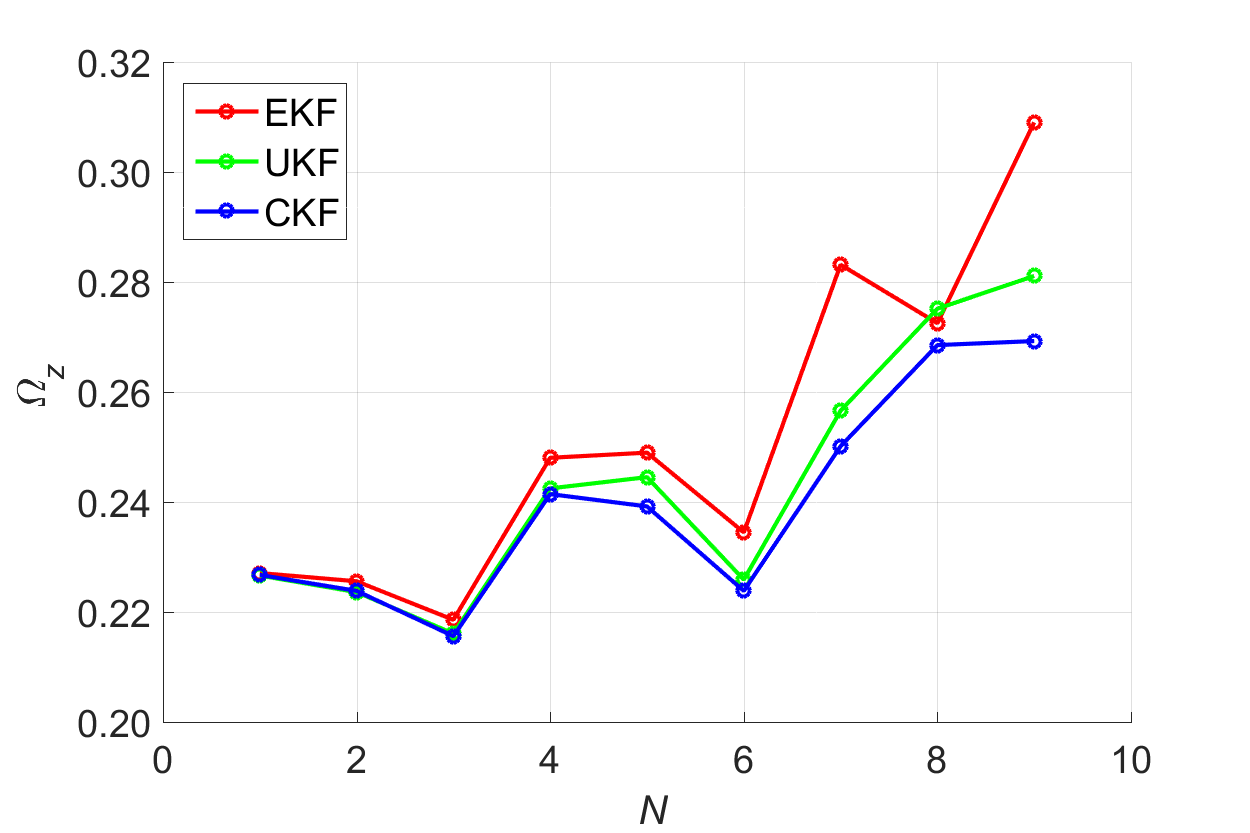
\includegraphics[height=0.2\textheight]{estcmpr_4} \\ б)}
	\end{minipage}
	\caption{Сравнение производительности алгоритмов фильтрации}
    \label{fig:est_cmpr}
\end{figure}

Превосходство UKF и CKF над EKF в этом экспериминте
обусловлено использованием в последнем из алгоритмов
линеаризованного уравнения стохастической дифференциальной системы \eqref{eq:m_dyn},
что негативно влияет на производительность метода при росте интервала измерений. Таким образом для системы управления квадрокоптером с поворотными роторами выбран кубатурный фильтр Калмана.

\section{Использование алгоритмов оценки состояния для идентификации параметров БЛА}

Эффективность работы системы управления напрямую зависит от качества оценки параметров динамики БЛА.
Если используемый регулятор не расчитан на работу в условиях неопределнности, ошибки в значениях используемых в системе управления ключевых констант могут привести к увеличению времени сходимости траектории к целевой, статическим ошибкам или даже потере устойчивости.
Так как в исследовании в основе контура управления лежит ПД-регулятор \ref{eq:m_reg}, необходимо как можно лучше идентифицировать параметры модели. 

Некоторые из динамических свойств объекта, такие как общая масса или физические размеры, измерить достаточно просто, для измерения других параметров требуется проводить достаточно трудоемкие операции.
Например, чтобы определить аэродинамические коэффициенты пропеллеров
$k$ и $b$
из выражений для внешних сил и моментов \ref{eq:m_dyn}, действующих на БЛА,
нужно демонтировать двигатель и использовать специальный стенд; такой способ применяют, например, в работе \cite{Ryll01}. При этом, например из-за микроповреждений пропеллеров, со временем эти параметры неизбежно изменятся и операцию придется повторять снова.

Отличной альтернативой является использование расширенного фильтра Калмана, с помощью которого возможно определять или уточнять некоторые параметры динамики квадрокоптера. Например, чтобы оценить аэродинамические константы $k$ и $b$, используем их как составляющие вектора состояния, вместе со скоростью и угловой скоростью:
\begin{equation}
\bm x = (\bm v^I, \bm \Omega^B, k, b)^T.
\end{equation}
При этом в качестве вектора измерений будем использовать
\begin{equation}
\bm z = (\bm v^I, \bm \Omega^B, \dot{\bm v^I}, \dot{\bm \Omega^B})^T.
\end{equation}
Как показывают эксперименты, в результате простого маневра -- взлета и разворота на $\frac{\pi}{2}$, который аппарат сможет выполнить относительно успешно даже с приблизительно известными параметрами, оценка коэффициентов $k$ и $b$
сходится к реальной. Известные параметры модели перечислены в Таблице \ref{tb:observer_params} , графики, демонстрирующие сходимость оценки к реальным значениям на рисунке \ref{fig:observer_k_b}, где красной линией изображена оценка, зеленой -- начальное приблизительное значение, синей -- истинное значение модели.
\begin{figure}[h!]
	\centering
	\subfloat[Оценка аэродинамического коэффициента пропеллера $k$]{%
		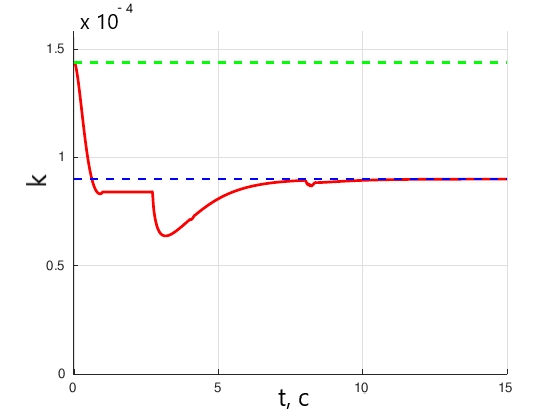
\includegraphics[clip,width=0.44\columnwidth]{k}%
	}
	\quad
	\subfloat[Оценка аэродинамического коэффициента пропеллера $b$]{%
		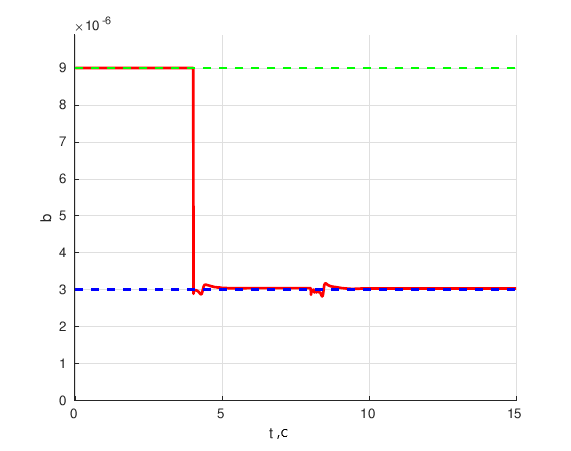
\includegraphics[clip,width=0.44\columnwidth]{b}%
	}
	\caption{ -- Уточнение параметров динамики БЛА}
	\label{fig:observer_k_b}
\end{figure}
\begin{table}[ht]
	\centering
	\caption{ -- Известные параметры модели}\label{tb:observer_params} 
	\begin{tabular}{lcl}
		\hline
		Параметр & Обозначение & Значение  \\\hline
		Общая масса & $M$ & 3,6 кг  \\
		Тензор инерции корпуса & $\bm J_B$ & $diag(53, 63, 98) \cdot{10^{-3}}$ кг$\cdot$м$^2$  \\
		Тензор инерции ротора & $\bm J_R$ & $diag(85, 85, 46) \cdot{10^{-6}}$ кг$\cdot$м$^2$  \\
		Миделево сечение корпуса & $S_{\perp}$ & 0,2 м$^2$ \\
		Луч & $L$ & 0,35 м \\
		Аэродинамический коэффициент & $C$ & 1,05\\	
		Максимальные обороты & $\tilde \omega_{max}$ & 500 рад/с \\		
		Максимальный угол & $\theta_{max}$ & ${\pi}/{4}$ рад \\
		\hline
	\end{tabular}
\end{table}
